% ============================================================
%  RFTIC — Representational Flexibility Theory of Insight Capacity
%  LaTeX Source — Production Version
%  Author: Miguel Marmore
%  Target: PsyArXiv preprint
% ============================================================

\documentclass[a4paper,twocolumn,10pt]{article}

% ── PACKAGES ────────────────────────────────────────────────
\usepackage[T1]{fontenc}
\usepackage[utf8]{inputenc}
\usepackage{lmodern}
\usepackage[a4paper, margin=1in, columnsep=0.25in]{geometry}
\usepackage{amsmath, amssymb, amsthm}
\usepackage{microtype}
\usepackage{booktabs}
\usepackage{graphicx}
\usepackage{xcolor}
\usepackage{xurl}
\usepackage{hyperref}
\usepackage{natbib}
\usepackage{authblk}
\usepackage{abstract}
\usepackage{titlesec}
\usepackage{enumitem}
\usepackage{float}
\usepackage{algorithm}
\usepackage{algpseudocode}

% ── HYPERREF CONFIG ─────────────────────────────────────────
\hypersetup{
  colorlinks = true,
  linkcolor  = black,
  citecolor  = black,
  urlcolor   = black,
  hypertexnames = false,
  pdftitle = {The Architecture of Insight: A Reduced-Model Hypothesis for Representational Flexibility and Insight Capacity},
}

% ── THEOREM ENVIRONMENTS ────────────────────────────────────
\newtheorem{theorem}{Theorem}
\newtheorem{proposition}{Proposition}
\newtheorem{corollary}{Corollary}
\newtheorem{lemma}{Lemma}

% ── SECTION FORMATTING ──────────────────────────────────────
\titleformat{\section}{\normalfont\bfseries\large}{\thesection.}{0.5em}{}
\titleformat{\subsection}{\normalfont\bfseries\normalsize}{\thesubsection.}{0.5em}{}
\titleformat{\subsubsection}{\normalfont\itshape\normalsize}{\thesubsubsection.}{0.5em}{}

% ── ABSTRACT FORMATTING ─────────────────────────────────────
\renewcommand{\abstractnamefont}{\normalfont\bfseries}
\renewcommand{\abstracttextfont}{\small}
\setlength{\absleftindent}{0pt}
\setlength{\absrightindent}{0pt}

% ── MATH SHORTCUTS ──────────────────────────────────────────
\newcommand{\eps}{\varepsilon}
\newcommand{\dE}{\Delta E}
\newcommand{\Ssaddle}{S_{\mathrm{saddle}}}
\newcommand{\psiA}{\psi_A}
\newcommand{\psiB}{\psi_B}
\newcommand{\WAB}{\tilde{W}_{AB}}

% ============================================================
\begin{document}
% ============================================================

% ── TITLE ───────────────────────────────────────────────────
\title{\textbf{The Architecture of Insight:\\
A Reduced-Model Hypothesis for Representational Flexibility and Insight Capacity}}

\author{Miguel Marmore}
\affil{Gama, Distrito Federal, Brazil\\
\texttt{miguelmarmore19@gmail.com}}

\date{}

% ── TITLE + ABSTRACT SPANNING BOTH COLUMNS ───────────
\twocolumn[
  \begin{@twocolumnfalse}
    \maketitle
    \begin{abstract}
    Insight---the sudden restructuring of a problem representation that yields a novel
    solution---has been associated with state-dependent factors including affect and attentional
    conditions. We introduce the \textbf{Representational Flexibility Theory of Insight
    Capacity} (RFTIC), a hypothesis that separates such state variables from a putative structural
    property of semantic connectivity. Within a reduced continuous-Hopfield model
    \citep{hopfield1982neural, hopfield1984graded}, orthonormal domain patterns and hypothesis (A1) imply the
    exact raw-eigenvalue shift $\lambda_W(\eps)=\lambda_{W0}-\eps$. With
    $\mu(\eps)=\lambda_W(\eps)-1=\mu_0-\eps$, $\mu_0=\lambda_{W0}-1>0$, and the additional
    transverse-gap hypothesis (A2), partial minimization of the Hopfield energy gives an asymptotic
    normal form near $\mu\to0^+$. Its quartic truncation has coefficient
    $g=\sum_i(v_i^*)^4$, minima $x_\pm=\pm\sqrt{3\mu/g}$, barrier
    $\dE(\eps)=3(\mu_0-\eps)^2/(4g)$, and critical value
    $\eps_{\mathrm{crit}}=\mu_0=\lambda_{W0}-1$. The order parameter vanishes with mean-field
    exponent $\beta=1/2$ as the two wells merge; above the critical point the reduced potential is
    single-welled, so a basin-to-basin escape rate is no longer the relevant observable. We validate
    the internal numerical implementation of the canonical normal-form dynamics using 16 values of
    $r=\dE/T$ and 6,000 trajectories per value. At moderate-to-high barriers, the stabilized
    conditional hazard agrees closely with the inverse one-dimensional MFPT. At lower barriers,
    the two estimands differ. Kramers' formula progressively approaches the inverse MFPT at high
    barriers. These results establish consistency of the
    reduced model only; they do not validate its proposed cognitive, clinical, or
    artificial-intelligence interpretations.

    \noindent\textbf{Keywords:} insight; representational flexibility; Kramers escape rate;
    Hopfield network; first-passage time; reduced stochastic model
    \end{abstract}
    \vspace{2em}
  \end{@twocolumnfalse}
]

% ============================================================
\section{Introduction}
% ============================================================

\subsection{State-Dependent Findings and an Explanatory Gap}

Insight performance has been associated with several task- and state-dependent factors, including
positive affect and patterns of attentional or executive engagement \citep{subramaniam2009positive,
kounios2014neuroscience}. The literature does not establish a single universal state of reduced
analytical control, and effects must be interpreted in relation to the specific task and manipulation.
In verbal insight tasks, \citet{jungbeeman2004neural} observed greater right anterior superior
temporal activity for insight than noninsight solutions and a right-temporal gamma-band increase
beginning approximately 300 milliseconds before the button-press response. These findings do not by
themselves demonstrate global prefrontal suppression, Default Mode Network activation, or that the
gamma increase precedes the first conscious awareness of the solution.

Performance and reported Aha experiences vary across tasks and individuals
\citep{danek2014magic,webb2018aha}. Established predictors are also important:
\citet{chuderski2018aha} found that working-memory capacity and reasoning were strongly related to
insight performance. RFTIC therefore proposes an additional candidate construct rather than assuming
an already isolated residual factor. Its incremental predictive validity must be tested against
working memory, reasoning, prior knowledge, task characteristics, and momentary state.

We term this hypothesized individual-level construct \emph{representational flexibility} (FR): the
putative capacity to encode the same problem under multiple representations and to transition between
them. The central hypothesis is that FR may contribute to \emph{insight capacity}---as distinct from
insight probability in a given moment. Whether FR is stable, trainable, measurable independently of
behavioral outcomes, or separable from established cognitive predictors remains an empirical
question.

\subsection{The Representational Change Theory and Its Limits}

The theoretical framework most directly relevant to our proposal is Ohlsson's Representational
Change Theory \citep[RCT;][]{ohlsson1992insight, ohlsson2011deep}. RCT proposes that insight occurs through
two mechanisms: \emph{constraint relaxation} (the softening of self-imposed problem framings) and
\emph{chunk decomposition} (the disaggregation of perceptual or conceptual units that block
alternative encodings). These mechanisms were tested in the original matchstick-arithmetic
experiments of \citet{knoblich1999constraint}, with related processes subsequently examined in other
insight tasks \citep{knoblich2001eyemovement,ollinger2008mentalset,ollinger2014ninedot,
danek2020closing}. RCT is thus a prominent process-level account of insight rather than an exclusive
or complete account of every insight phenomenon.

RCT describes representational operations associated with the transition from impasse to solution.
RFTIC introduces a complementary level of analysis concerned with how a model's transition propensity
might vary across systems or individuals. The distinction between a theory of an event and a theory
of a proposed capacity is our conceptual framing, not a claim that RCT explicitly excludes
individual differences.

This is not a criticism of the theory's internal logic but a recognition of a different level of
analysis. The relationship is analogous to that between the kinematics of chemical reactions---which
describes bond-breaking and bond-forming sequences---and transition-state theory, which predicts
\emph{rates} as a function of energy barriers and fluctuations. RCT motivates the representational
operations; RFTIC proposes a statistical-mechanical layer in which a specified perturbation changes
a reduced transition barrier. Whether this formalism explains stable human differences in insight
is an open empirical question.

\subsection{State-Based Accounts and the Friston Constraint}

A parallel literature develops the Free Energy Principle and active-inference accounts of
perception, action, and, in specific formal models, curiosity and insight
\citep{friston2010freeenergy,friston2017activeinference}. RFTIC uses a distinct stochastic model:
active-inference precision and the RFTIC noise parameter $T$ are not established as mathematically or
empirically identical, and no cited evidence shows that dopamine controls RFTIC-like exploration.

RFTIC asks a complementary structural question: whether prior connection weights retain
training-induced changes that affect later representational transitions. In the reduced stochastic
model, $T$ controls noise amplitude while $\eps$ changes the potential. Treating these mathematical
parameters as neural precision and learned semantic connectivity is an interpretive hypothesis, and their
empirical independence has not been established.

\subsection{The Trainability Gap}

A third line of evidence concerns procedures that can facilitate performance on insight-related
tasks. In controlled studies, explicit representational-change procedures improved performance on
previously untrained verbal insight problems \citep{patrick2014training,patrick2015representation};
\citet{patrick2015representation} also observed an advantage in an independent trained group tested
after 48 hours. This is within-class procedural generalization, not a longitudinal retention curve,
far transfer, stable trait change, or evidence of altered neural connectivity. Analogical comparison
can facilitate access to structurally related solutions \citep{gick1983analogy,kurtz2007analogy},
and brief mindfulness manipulations have also been studied with insight tasks
\citep{ostafin2012mindfulness}. These findings motivate candidate interventions but do not establish
a single latent FR variable or a common biological mechanism.

RFTIC proposes an organizing framework. The six components in Section~\ref{sec:framework} organize
candidate interventions by their hypothesized effects on $W$, trajectories, or $T$. Existing
training studies motivate these candidates but do not establish a single latent variable or the
specific network changes assumed by the model.

\subsection{The Present Paper}

We proceed as follows. Section~\ref{sec:framework} defines FR as a hypothesis and organizes six
candidate components with proposed model-level mappings.
Section~\ref{sec:math} states the assumptions and derives the chain
$W(\eps)\to\lambda_W(\eps)\to\mu(\eps)\to U(x;\eps)\to\dE(\eps)\to k\to P_\tau$.
Section~\ref{sec:simulation} compares Euler--Maruyama simulation with an exact one-dimensional
first-passage calculation and the Kramers asymptotic limit. Section~\ref{sec:discussion} separates
predictions of this reduced model from speculative cognitive, clinical, and artificial-intelligence
implications.

The argument of this paper rests on a single conceptual inversion: the literature has asked,
\emph{what states facilitate insight?} We ask, \emph{what structural properties might contribute
to representational transition capacity beyond transient state-dependent variation?} The second motivates a
complementary level of analysis focused on capacity rather than a single insight event.

% ============================================================
\section{The RFTIC Framework}
\label{sec:framework}
% ============================================================

\subsection{Definition and Scope}

Representational flexibility (FR) is defined within RFTIC as a hypothesized individual-level
construct concerning connectivity across representational domains. Participant-specific semantic
association networks can in principle be estimated from suitable behavioral data, and group-level
topological differences have been studied in related creativity research
\citep{kenett2014networks,zemla2018estimating}. We therefore propose that within- and across-domain
network structure may provide candidate operationalizations of FR. Corpus-trained Word2Vec, GloVe,
and BERT representations provide exploratory geometric spaces
\citep{mikolov2013distributed,pennington2014glove,devlin2019bert}, but they do not measure a
person's mind. Cosine distance is not a validated FR measure, and semantic embedding geometry is not
psychological FR by definition.

In the reduced model, the hypothesized structural contribution is parameterized by a nonnegative
scalar $\eps$, designated the \textbf{Topological Flexibility Index (TFI)}. TFI is a proposed model
parameter rather than a validated psychometric variable, and $\eps$ has not been empirically
calibrated from any network or embedding metric. The double-well regime exists only for
$0\leq\eps<\eps_{\mathrm{crit}}$, where
$\eps_{\mathrm{crit}}=\mu_0=\lambda_{W0}-1$ is derived in Section~\ref{sec:math}; this mathematical interval is not an empirically calibrated
cognitive scale.

This proposed measurement strategy is intended to avoid the central tautology that threatens any capacity-based theory
of insight: if FR were defined as ``the tendency to change representations successfully,'' and
insight as ``successful representational change,'' the argument would be circular. By grounding FR
in participant-level network descriptors estimated independently of the target problem-solving
episode, future studies could test reliability, construct validity, and incremental prediction rather
than defining the construct by the outcome it is intended to explain.

\subsection{Six Components of Representational Flexibility}

We propose six candidate components and intervention targets that may influence representational
flexibility through distinct psychological processes. Their assignments to $W$, search trajectories,
and $T$ are explanatory modeling choices, not findings of the cited experiments.

\textbf{Component 1 --- Inconsistency Detection.}
Inconsistency-evaluation procedures have been tested as ways to cue re-encoding during verbal insight
problem solving \citep{patrick2014training,patrick2015representation}. We hypothesize, without
direct neural evidence, that repeated use of such a procedure could be represented by a selected
connectivity update in $W_{AB}$, by analogy with Hebbian learning
\citep{hebb1949organization}.

\textbf{Component 2 --- Cross-Domain Analogical Transfer.}
Research on analogical comparison and transfer motivates the hypothesis that practice in cross-domain
mappings could change effective associative structure \citep{gick1983analogy,kurtz2007analogy}.
The modeled update $\WAB = \eps(\psiA\psiB^T + \psiB\psiA^T)$ is the perturbation analyzed in
Theorem~\ref{thm:shift}; it is an RFTIC modeling assumption, not a connectivity equation inferred
from those experiments.

\textbf{Component 3 --- Tolerance of Impasse.}
A candidate capacity to sustain representational ambiguity without premature closure. Direct
intervention evidence is not established here. In the model analogy, Component 3 changes the
available observation or search time rather than $W$ itself.

\textbf{Component 4 --- Metacognition of Impasse.}
A proposed capacity to distinguish representational impasse from analytic difficulty. Foundational
metacognitive accounts motivate monitoring and control concepts
\citep{flavell1979metacognition,nelson1990metamemory}, but they do not establish an
RFTIC-specific impasse classifier. Such classification is hypothesized to direct exploratory effort
toward representational change when impasse is genuine.

\textbf{Component 5 --- Type~1 Disinhibition.}
Transient relaxation of habitual analytic monitoring is considered as a candidate intervention
target. The Type~1 terminology is descriptive \citep{kahneman2011thinking}, and mindfulness
research provides a task-level precedent rather than evidence of voluntary prefrontal suppression
\citep{ostafin2012mindfulness}. Within RFTIC, Component 5 is represented as a transient change in
$T$ rather than in $W$; this theoretical mapping does not identify $T$ with neural precision.

\textbf{Component 6 --- Chunk Decomposition.}
The trained capacity to disaggregate perceptual or conceptual units fused through expertise or
habit \citep{knoblich1999constraint}. The model maps chunk decomposition to changes in the intra-domain blocks
$W_{AA}$ and $W_{BB}$ and hence to the raw baseline eigenvalue $\lambda_{W0}$ and net coefficient
$\mu_0=\lambda_{W0}-1$. Within the truncated normal form, changing $\mu_0$ changes both
$\dE=3(\mu_0-\eps)^2/(4g)$ and the critical point; the proposed neural mapping has not been
demonstrated, and no cited study shows a stable training-induced modification of neural $W$.

\subsection{Summary: Coordinated Structural Modification}

Table~\ref{tab:components} summarizes the proposed components, candidate intervention targets, and
hypothesized model-level mappings.

\begin{table*}[htbp]
\centering
\caption{Proposed RFTIC components, candidate intervention targets, and hypothesized model-level mappings.}
\label{tab:components}
\small
\begin{tabular}{@{}llll@{}}
\toprule
\textbf{Component} & \textbf{Target} & \textbf{Candidate mechanism} & \textbf{Hypothesized model effect} \\
\midrule
1 --- Inconsistency Det. & $W_{AB}$ & Sparse Hebbian & $\uparrow \eps$ (targeted) \\
2 --- Analogical Transfer & $W_{AB}$ & Structured Hebbian & $\uparrow \eps$ (aligned) \\
3 --- Impasse Tolerance & Trajectory & Dwell-time extension & Longer search window $\tau$ \\
4 --- Metacognition & Trajectory & Routing optimization & Effective search window $\tau$ \\
5 --- Type~1 Disinhibition & $T$ & Monitoring shift & $\uparrow T$ (transient) \\
6 --- Chunk Decomp. & $W_{AA}$, $W_{BB}$ & Intra-domain weakening & $\downarrow \mu_0 \to \downarrow \dE$ \\
\bottomrule
\end{tabular}
\end{table*}

In the proposed mapping, Components 1, 2, and 6 act on structural parameters; Components 3 and 4
act on search trajectories; and Component 5 acts on $T$. These categories are modeling hypotheses
rather than established biological mechanisms.

% ============================================================
\section{Mathematical Formulation}
\label{sec:math}
% ============================================================

\subsection{Network, transition mode, and training perturbation}

Let $S\in\mathbb{R}^N$ be a continuous activation vector and let the symmetric matrix
$W\in\mathbb{R}^{N\times N}$ encode the semantic connectivity. The bilinear Hopfield energy is
\begin{equation}
E(S)=-\tfrac12 S^TWS,
\label{eq:energy}
\end{equation}
with the domain partition
\begin{equation}
W=\begin{pmatrix}W_{AA}&W_{AB}\\W_{BA}&W_{BB}\end{pmatrix},
\qquad W_{AB}=W_{BA}^T.
\label{eq:blocks}
\end{equation}
RFTIC denotes the proposed psychological capacity by representational flexibility (FR). Its model
parameter, the Topological Flexibility Index (TFI), is $\eps\geq0$; FR and $\eps$ are therefore not
interchangeable quantities. Let the two domain patterns satisfy
\begin{equation}
\|\psiA\|=\|\psiB\|=1,\qquad \psiA^T\psiB=0,
\label{eq:orthonormal}
\end{equation}
and define the normalized contrastive direction, its symmetric companion, the transverse space,
and the reduced coordinate by
\begin{equation}
\begin{aligned}
v^*&=\frac{\psiA-\psiB}{\sqrt2},&
u&=\frac{\psiA+\psiB}{\sqrt2},\\
V_\perp&=\{w:w^Tv^*=0\},& x&=v^{*T}S.
\end{aligned}
\label{eq:projection}
\end{equation}
$\psiA$ and $\psiB$ define the contrastive direction used to construct the transition mode, whereas
the minima of the reduced normal form represent effective states along that coordinate rather than
the original pattern vectors themselves.
The cross-domain Hebbian perturbation is
\begin{equation}
\begin{aligned}
\WAB(\eps)&=\eps(\psiA\psiB^T+\psiB\psiA^T),\\
W(\eps)&=W_0+\WAB(\eps).
\end{aligned}
\label{eq:hebbian}
\end{equation}

\begin{lemma}[Action of the training term]
\label{lem:training}
Under \eqref{eq:orthonormal}, $\WAB(\eps)v^*=-\eps v^*$.
\end{lemma}
\begin{proof}
Writing $a=\psiA$ and $b=\psiB$,
\begin{align*}
(ab^T+ba^T)\frac{a-b}{\sqrt2}
&=\frac{a[b^T(a-b)]+b[a^T(a-b)]}{\sqrt2}\\
&=\frac{-a+b}{\sqrt2}=-v^*.
\end{align*}
Multiplication by $\eps$ proves the statement.
\end{proof}

The reduction requires the following explicit baseline hypothesis:
\begin{equation}
\tag{A1}
\begin{aligned}
W_0v^*&=\lambda_{W0}v^*,& \lambda_{W0}&=v^{*T}W_0v^*,\\
\mu_0&:=\lambda_{W0}-1>0.&&
\end{aligned}
\label{eq:A1}
\end{equation}
Hypothesis~\eqref{eq:A1} concerns only $v^*$; it does not require $\psiA$ and $\psiB$ to be
individual eigenvectors or $W_0$ to be isotropic on their two-dimensional span.

\begin{theorem}[Exact shift along the transition mode]
\label{thm:shift}
Under \eqref{eq:orthonormal} and (A1), $v^*$ remains an eigenvector of $W(\eps)$ and
\begin{equation}
\begin{aligned}
\boxed{\lambda_W(\eps)=\lambda_{W0}-\eps},\\
\boxed{\mu(\eps):=\lambda_W(\eps)-1=\mu_0-\eps}.
\end{aligned}
\label{eq:eigenvalue_shift}
\end{equation}
\end{theorem}
\begin{proof}
By (A1) and Lemma~\ref{lem:training},
$W(\eps)v^*=W_0v^*+\WAB(\eps)v^*=(\lambda_{W0}-\eps)v^*$.
\end{proof}
Thus the coefficient of $\eps$ is fixed at one rather than fitted. Without (A1),
$v^{*T}W(\eps)v^*$ is a Rayleigh quotient, not necessarily an eigenvalue, and the neglected coupling
to directions orthogonal to $v^*$ becomes an additional approximation. The raw eigenvalue
$\lambda_W$ and the effective quadratic coefficient $\mu=\lambda_W-1$ are distinct; the unit shift
comes from the quadratic saturation term in the Hopfield energy.

The one-dimensional reduction additionally requires a uniform transverse gap on the interval
$I\subseteq[0,\eps_{\mathrm{crit}})$ under consideration:
\begin{equation}
\tag{A2}
\sup_{\eps\in I}\lambda_{\max}\!\left(W(\eps)\big|_{V_\perp}\right)\leq1-\gamma,
\qquad \gamma>0.
\label{eq:A2}
\end{equation}
Hypothesis (A2) is additional to (A1). It supplies transverse stability and convexity sufficient for
the reduction, but it has not been established for real semantic networks. A two-dimensional model
for cases in which the symmetric mode also becomes critical is outside the present scope.

\begin{lemma}[Transverse minimizer]
\label{lem:transverse}
Under (A1) and (A2), the Hopfield energy is uniformly strongly convex on each transverse slice. Near
$x=0$ there is a unique smooth minimizer $y^*(x)\in V_\perp$. It satisfies
$y^*(0)=0$ and $y^*(-x)=-y^*(x)$, with $y^*(x)=O(x^3)$.
\end{lemma}
The result follows from $D(S)\succeq I$ in the full Hessian
$H(S)=-W+D(S)$, the gap in (A2), and the implicit function theorem. A proof and the explicit slaving
coefficient are given in Supplementary Note S1.

\subsection{Reduced potential, barrier, and critical point}

Hopfield's graded-response model supplies a general inverse-transfer Lyapunov energy
\citep{hopfield1984graded}. For a tanh transfer function with the gain/resistance normalization
adopted here, symmetric weights, state/output identification, and zero external input, that general
energy reduces to the following normalized special case:
\begin{equation}
E_{\mathrm{Hopfield}}(S)=-\tfrac12S^TWS+
\sum_i\int_0^{S_i}\tanh^{-1}(s)\,ds.
\label{eq:hopfield_full}
\end{equation}
The local expansion
\begin{equation}
\int_0^z\tanh^{-1}(s)\,ds
=\frac{z^2}{2}+\frac{z^4}{12}+\frac{z^6}{30}+\mathcal{O}(z^8)
\label{eq:taylor}
\end{equation}
gives, on the line $S=xv^*$,
\begin{equation}
\begin{aligned}
\mathcal{S}(x)&:=\sum_i\int_0^{xv_i^*}\tanh^{-1}(s)\,ds,\\
\mathcal{S}(x)&=\frac{x^2}{2}+\frac{g}{12}x^4+\frac{h}{30}x^6
+\mathcal{O}(x^8),\\
g&:=\sum_i(v_i^*)^4,\qquad h:=\sum_i(v_i^*)^6.
\end{aligned}
\label{eq:saturation_mode}
\end{equation}
The $x^2/2$ contribution is the unit-leak shift: the quadratic coefficient is
$\mu=\lambda_W-1$, not the raw eigenvalue $\lambda_W$. For normalized $v^*$, $g$ is its inverse
participation ratio and satisfies $1/N\leq g\leq1$.

At Level A, define the reduced energy by partial minimization over the stable transverse directions,
\begin{equation}
U(x;\eps):=\min_{y\in V_\perp}E_{\mathrm{Hopfield}}(xv^*+y).
\label{eq:partial_minimization}
\end{equation}

\begin{proposition}[Asymptotic reduced normal form]
\label{prop:normal_form}
Under (A1)--(A2), for sufficiently small $|x|$,
\begin{equation}
U(x;\eps)=\frac{g}{12}x^4-\frac{\mu(\eps)}{2}x^2+c_6x^6+\mathcal{O}(x^8).
\label{eq:reduced_asymptotic}
\end{equation}
The transverse minimization first changes the line-restricted energy at order $x^6$; in particular,
it does not alter the quadratic or quartic coefficients.
\end{proposition}
The proof sketch inserts the slaving relation $y^*(x)=O(x^3)$ from
Lemma~\ref{lem:transverse} into the energy expansion and minimizes the resulting transverse
quadratic form. The formula for $c_6$, its bounds, and the full derivation are given in Supplementary
Note S2. Thus \eqref{eq:reduced_asymptotic} is an asymptotic reduction near the bifurcation, not an
exact finite-$\mu$ identity.

At Level B, the paper adopts the quartic truncation
\begin{equation}
U_{\mathrm{nf}}(x;\eps)=\frac{g}{12}x^4-\frac{\mu(\eps)}{2}x^2
\label{eq:doublewell}
\end{equation}
as the normal-form model for the barrier, Kramers rate, first-passage calculation, and simulation.
For $\mu>0$,
\begin{equation}
U_{\mathrm{nf}}'(x)=x\left(\frac{g}{3}x^2-\mu\right)=0,
\qquad x_\pm=\pm\sqrt{\frac{3\mu}{g}},
\label{eq:wells}
\end{equation}
where $x_\pm$ are minima and $x=0$ is the saddle. Direct substitution gives
\begin{equation}
\begin{aligned}
U_{\mathrm{nf}}(x_\pm)&=-\frac{3\mu^2}{4g},\\
\dE&=U_{\mathrm{nf}}(0)-U_{\mathrm{nf}}(x_\pm)=\frac{3\mu^2}{4g}.
\end{aligned}
\label{eq:barrier_lambda}
\end{equation}
Combining \eqref{eq:eigenvalue_shift} and \eqref{eq:barrier_lambda} gives the Level-B barrier law.
The interval displayed below identifies the double-well regime of the quartic model. Its accuracy
as an approximation to the Hopfield barrier is asymptotic near $\eps\to\mu_0^-$:
\begin{equation}
\boxed{\dE(\eps)=\frac{3(\mu_0-\eps)^2}{4g}},\qquad 0\leq\eps<\mu_0,
\label{eq:barrier}
\end{equation}
The deterministic critical point is
\begin{equation}
\boxed{\eps_{\mathrm{crit}}=\mu_0=\lambda_{W0}-1}.
\label{eq:critical}
\end{equation}
The order parameter is the well separation
\begin{equation}
M(\eps)=x_+-x_-=2\sqrt{\frac{3(\mu_0-\eps)}{g}}.
\label{eq:order_parameter}
\end{equation}
Hence $M\propto(\eps_{\mathrm{crit}}-\eps)^{1/2}$ and the reduced mean-field model has
$\beta=1/2$. This exponent coincides with the mean-field value from Landau theory for a continuous
transition in a quartic--quadratic potential \citep{landau1980statistical}. Without a renormalization-group
derivation, this coincidence does not establish that RFTIC shares a universality class with any
physical system.

As $\eps\to\eps_{\mathrm{crit}}^-$, the two minima merge at $x=0$. At the critical value,
$U_{\mathrm{nf}}(x)=gx^4/12$ has a single degenerate quartic minimum. For
$\eps>\eps_{\mathrm{crit}}$, the positive quadratic and quartic terms form a single well at the
origin, representing the quiescent state along the contrastive coordinate. In this regime the
normal form has no two distinct basins along that coordinate, so a basin-to-basin escape rate is
undefined rather than zero. The evenness $U(-x)=U(x)$ follows from the global sign symmetry
$E_{\mathrm{Hopfield}}(-S)=E_{\mathrm{Hopfield}}(S)$; it is not an independent double-well
assumption or an exchange symmetry between $\psiA$ and $\psiB$.

\subsection{Kramers rate and finite-window probability}
\label{sec:master}

Consider the overdamped Langevin dynamics with friction set to one,
\begin{equation}
dx=-U'(x)\,dt+\sqrt{2T}\,dW_t.
\label{eq:langevin}
\end{equation}
Here $x$ is the physical reduced coordinate and the mobility is set to one. For $\mu>0$,
$U_{\mathrm{nf}}''(0)=-\mu$ and $U_{\mathrm{nf}}''(x_\pm)=2\mu$.
Kramers' historical work provides the foundation for activated barrier escape
\citep{kramers1940brownian}; the expression used here is the corresponding modern overdamped
Eyring--Kramers specialization for a committed basin-to-basin transition:
\begin{equation}
\begin{aligned}
k(\eps,T)
&=\frac{\sqrt{U''(x_-)|U''(0)|}}{2\pi}e^{-\dE/T}\\
&=\frac{\mu(\eps)}{\sqrt2\,\pi}
\exp\!\left[-\frac{3\mu(\eps)^2}{4gT}\right].
\end{aligned}
\label{eq:kramers_full}
\end{equation}
The prefactor is independent of $T$ and $g$; those quantities enter the exponential through the
barrier ratio.
The quantity $k$ has units of inverse time and is not a probability. If the post-transient escape
process is approximately Poisson over an observation window $\tau$, the comparable finite-window
probability is
\begin{equation}
\boxed{P_\tau(\eps,T)=1-\exp[-k(\eps,T)\tau]}.
\label{eq:finite_window}
\end{equation}

\subsection{Dimensionless form and observables}

For $\mu>0$, introduce the canonically rescaled coordinate and time
$y=\sqrt{g/\mu}\,x$ and $s=\mu t$. Distinguish the physical noise $T$ from the effective
canonical noise
\begin{equation}
\theta:=\frac{gT}{\mu^2}=\frac{3}{4r},\qquad
r=\frac{\dE}{T}=\frac{3\mu^2}{4gT}.
\label{eq:r}
\end{equation}
Equation~\eqref{eq:langevin} becomes
\begin{equation}
dy=-\left(\frac{y^3}{3}-y\right)ds+\sqrt{\frac{3}{2r}}\,dW_s.
\label{eq:nondimensional_sde}
\end{equation}
Thus the dimensionless dynamics depend only on the invariant barrier ratio $r$: rescaling the
coordinate moves $g$ into the effective noise but does not change $\dE/T$. With
$\kappa=k/\mu$, the committed Kramers prediction is
\begin{equation}
\boxed{\kappa_K(r)=\frac{1}{\sqrt2\,\pi}e^{-r}}.
\label{eq:kappa_kramers}
\end{equation}
Kramers' formula is asymptotic as $r\to\infty$; $r=1$ is not a sharp validity boundary.

Two stopping observables must be distinguished. Starting at $x_0=x_-=-x_+$,
\begin{equation}
\begin{aligned}
\tau_{\mathrm{hit}}&=\inf\{t:x(t)\geq0\},\\
\tau_{\mathrm{commit}}&=\inf\{t:x(t)\geq x_+\}.
\end{aligned}
\label{eq:hit_commit}
\end{equation}
For boundaries $a=-x_+$ and $b=x_+$, the one-dimensional committor is
\begin{equation}
q(x_0)=\frac{\int_a^{x_0}e^{U(y)/T}\,dy}{\int_a^b e^{U(y)/T}\,dy},
\label{eq:committor}
\end{equation}
so the evenness inherited from $E(-S)=E(S)$ gives $q(0)=1/2$: reaching the saddle is not yet a committed transition. The
half-Gaussian saddle integral implies
\begin{equation}
k_{\mathrm{hit}}/k_{\mathrm{commit}}\longrightarrow2
\quad\text{as }r\to\infty.
\label{eq:hit_commit_ratio}
\end{equation}
The old intermediate threshold measured a different observable. Once the absorbing boundary is the
mirror well $x_+$, no reactive-flux or Grote--Hynes correction is required for this overdamped
one-dimensional comparison.

% ============================================================
\section{Numerical Validation of the Reduced Model}
\label{sec:simulation}
% ============================================================

\subsection{Model, implementation, and reference calculations}

The mathematical model is Equation~\eqref{eq:nondimensional_sde}; the numerical implementation is
its Euler--Maruyama discretization. Each trajectory starts at $y_0=-\sqrt3$ and is counted as a
committed transition only on first reaching $+\sqrt3$. This definition matches the basin-to-basin
observable in Equation~\eqref{eq:kramers_full}, rather than first arrival at the saddle.
Section~\ref{sec:simulation} validates the canonical one-dimensional normal-form dynamics and its
first-passage implementation; it does not validate the finite-$\mu$ Hopfield landscape, the
stochastic dimensional reduction, or the cognitive interpretation.

The production sweep used 16 log-spaced values $r\in[0.15,7.0]$, canonical noise
$\theta=gT/\mu^2=3/(4r)$,
$\Delta s=0.01$, and a maximum window $s_{\max}=150$. Exactly 6,000 trajectories were run at each
point (96,000 total). The seed bases were $77{,}000+10{,}000i$, $i=0,\ldots,15$, and are archived
with the data. The code contained a mechanism to add batches until 100 events were observed, but
the initial 6,000 trajectories already exceeded this target at all points; consequently, no
adaptive increase occurred in the production sweep.

Trajectories without a transition by $s_{\max}$ were right-censored. For $d$ observed events, the
constant-hazard estimate was
\begin{equation}
\widehat\kappa=\frac{d}{\sum_i t_i^{\mathrm{obs}}+n_{\mathrm{cens}}s_{\max}}.
\label{eq:censored_mle}
\end{equation}
The initial relaxation transient was handled by conditioning on survival to a candidate $t^*$,
discarding earlier events, re-baselining the remaining times to $t-t^*$, and refitting
Equation~\eqref{eq:censored_mle}. Candidates were
$\{0,0.5,1,2,4,8,16,32\}T_{\mathrm{relax}}$, with
$T_{\mathrm{relax}}=[U''(y_-)]^{-1}=0.5$ in canonical units. The internal reference was the estimate at the largest
candidate retaining at least 20 events. The selected $t^*$ was the smallest candidate within 5\%
of that reference. This rule used only the empirical escape-time data, not the exact first-passage
or Kramers values.

After selecting $t^*$, estimation was conditioned on survival to $t^*$. For this post-truncation
set, $\widehat\kappa=d_{\mathrm{post}}/\mathcal{T}_{\mathrm{post}}$, where
$d_{\mathrm{post}}$ is the number of committed transitions observed after left truncation and
$\mathcal{T}_{\mathrm{post}}$ is the corresponding total time at risk, including right-censored
survivors. The reported approximate 95\% interval is
$\widehat\kappa\exp(\pm1.96/\sqrt{d_{\mathrm{post}}})$.
This fit estimates a constant escape hazard over the post-$t^*$ window conditional on survival
to $t^*$.

For an independent one-dimensional reference, the exact first-passage expression from the backward
equation was evaluated numerically. The nested quadrature follows from the standard one-dimensional
backward first-passage formulation, specialized here to the present drift, diffusion, and
reflecting/absorbing boundary conventions \citep{szabo1980firstpassage}:
\begin{equation}
\tau(y_0\!\to b)=\frac1\theta\int_{y_0}^{b} e^{\mathcal{U}(v)/\theta}
\left[\int_a^v e^{-\mathcal{U}(z)/\theta}\,dz\right]dv,
\label{eq:exact_mfpt}
\end{equation}
where $\mathcal{U}(y)=y^4/12-y^2/2$, with $y_0=-\sqrt3$, absorbing $b=+\sqrt3$, and $a=-20$ as a numerical representation of the confining
boundary at $-\infty$. We denote the inverse point-start MFPT by
$\kappa_{\mathrm{exact}}=1/\tau$. The mean includes the initial transient of the complete
first-passage distribution. Close agreement with the stabilized hazard is expected when local
relaxation is rapid relative to escape and first-passage times are approximately exponential.
The MFPT expression is exact within the reduced one-dimensional boundary-value
problem, apart from the separately checked finite grid and cutoff; it is not an exact solution of
the full Hopfield network. The Kramers curve, Equation~\eqref{eq:kappa_kramers}, is a distinct
high-barrier asymptotic approximation.

\subsection{Convergence and statistical safeguards}

At $r=3.5$, varying the quadrature grid from 5,000 to 80,000 points and the lower cutoff from
$-15$ to $-30$ left $\kappa_{\mathrm{exact}}=0.005829$ unchanged to six significant figures
(variation below 0.01\%). The archived Euler--Maruyama step-size check used
$\Delta s=0.02,0.01,0.005$ at $r\approx1,3.5,7$. Only a summary was retained for the two
lower-barrier points. At $r=7$, a re-test with approximately 150
events per step size gave $\widehat\kappa=0.000205$, $0.000198$, and $0.000183$, respectively;
the 3--8\% changes were comparable to the approximately 8\% relative Monte Carlo standard errors.
These checks were limited to the three representative points.

As an additional censoring-window sensitivity check, doubling the maximum canonical observation
window from $s_{\max}=150$ to $300$ changed the stabilized rate estimates by approximately 1.5\%,
1.8\%, 4.7\%, and 5.5\% at $r\approx3.25,4.19,5.42$, and $7.0$, respectively. Sensitivity was
therefore modest but nonzero and increased toward the most strongly censored high-barrier conditions.

As a diagnostic of the observable definition, the empirical
$\kappa_{\mathrm{hit}}/\kappa_{\mathrm{commit}}$ ratios at
$r=1,2,3.5,5,7$ were $2.41,2.12,2.00,2.03,2.09$, respectively, approaching the asymptotic factor
of two in Equation~\eqref{eq:hit_commit_ratio}. This isolates the former saddle-hit discrepancy as
an observable mismatch rather than evidence for an additional dynamical correction.

\subsection{Results}

Figure~\ref{fig:validation} shows the three-way comparison. For $r\geq2.5$, the stabilized
simulation estimate and inverse MFPT differ by approximately 0.5--3\%, and the inverse MFPT lies
within the reported simulation interval at all five tested points in this regime. At lower
barriers, the stabilized estimate is systematically higher than the point-start inverse MFPT.
With appreciably non-exponential first-passage times, these are different estimands, so their
discrepancy does not measure integration error.
Kramers' expression is poor at low barriers, captures the scale at intermediate $r$, and approaches
the exact rate progressively at high $r$. At $r=7$, the stabilized simulation estimate is
$0.000193$ (95\% CI $[0.000166,0.000225]$), the exact first-passage rate is $0.000192$, and the
Kramers rate is $0.000205$. Thus Kramers' rate formula emerges progressively as the high-barrier
asymptotic limit of the exact first-passage dynamics, with a residual, shrinking discrepancy at the
$r$ values tested here.

The log-ratio $\log(\kappa_{\mathrm{exact}}/\kappa_K)$ decreases in magnitude to approximately
$-0.066$ at $r=7$. A post hoc regression over $r\geq1.5$ was consistent with an $O(1/r)$ correction
($R^2=0.86$) but had a nonzero intercept of approximately $-0.046$; this pattern is descriptive and
does not establish the correction order. The hazard procedure selected no truncation at several
moderate-to-high barrier points, where the stabilized and untruncated estimates coincide by
construction. Their relative difference was 0.34\% at $r=7$.

Complete numerical values for all 16 sweep points are reported in Supplementary Table S1.

\begin{figure*}[htbp]
\centering
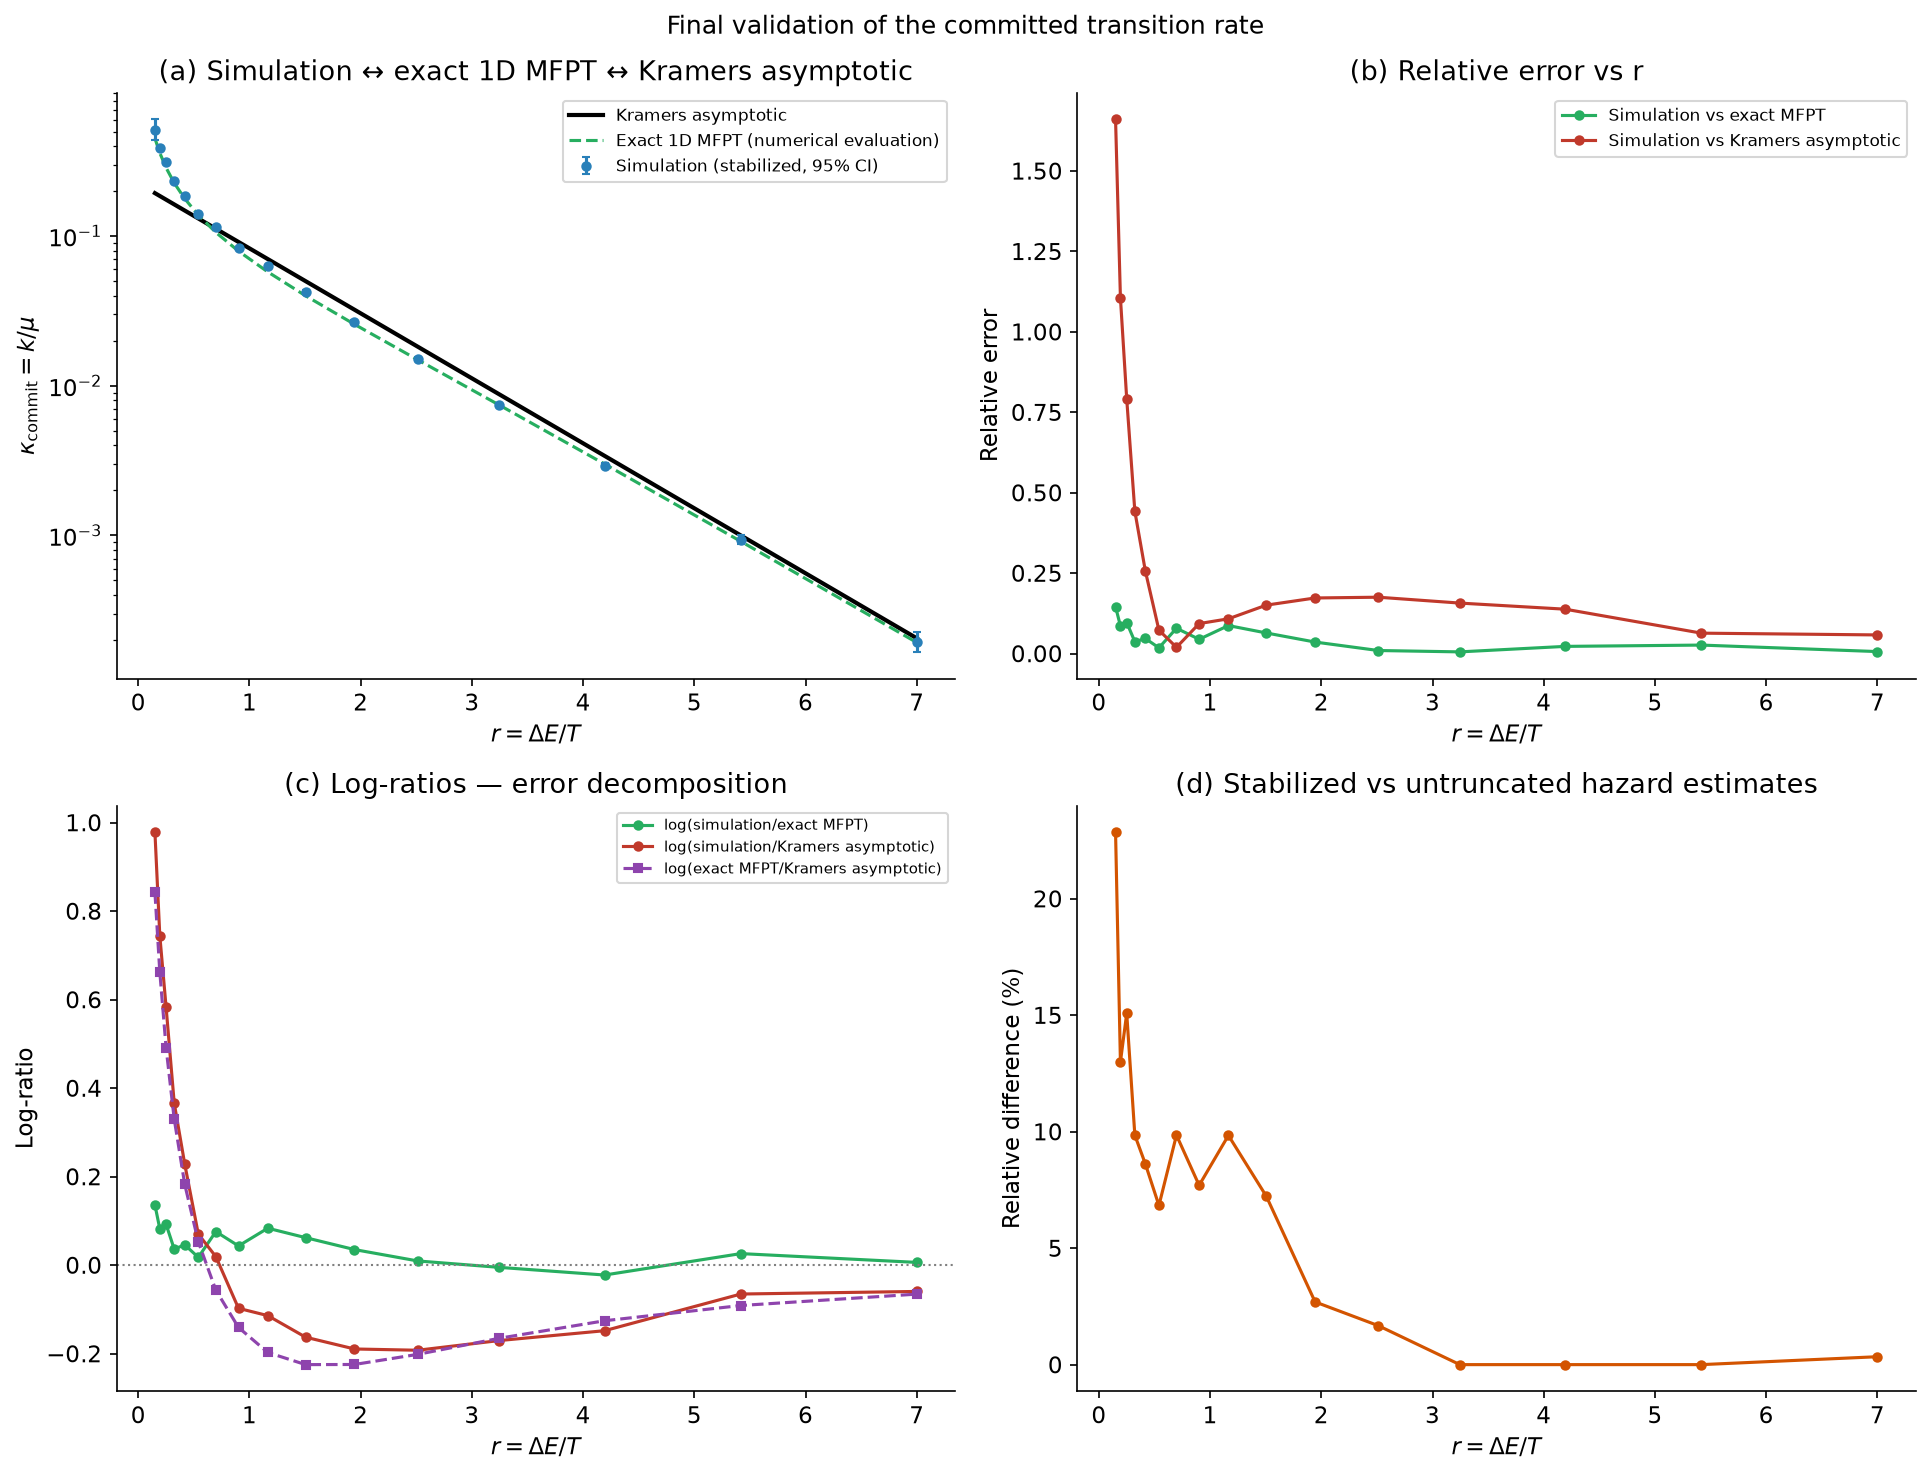
\includegraphics[width=\textwidth]{../figures/figure1_final_validation.png}
\caption{Validation of the committed basin-to-basin rate across
$r=\Delta E/T$. (a) Hazard-stabilized simulation estimates with right-censoring and approximate
95\% confidence intervals, the numerically evaluated inverse point-start MFPT, and the Kramers
asymptotic formula. (b) Absolute relative differences between the stabilized estimate and each
reference. At low barriers the stabilized hazard and inverse MFPT target distinct quantities.
(c) Log-ratios separating the stabilized--MFPT and MFPT--Kramers differences.
(d) Absolute difference between the stabilized and untruncated hazard estimates, expressed as
a percentage of the untruncated estimate.}
\label{fig:validation}
\end{figure*}

% ============================================================
\section{Discussion}
\label{sec:discussion}
% ============================================================

\subsection{Interpretation of the critical regime}

Within the truncated normal form, increasing $\eps$ toward $\eps_{\mathrm{crit}}$ decreases the
separation between two energetically equivalent effective states along the contrastive coordinate.
At $\eps_{\mathrm{crit}}$ they coalesce; above it, the potential is single-welled at the quiescent
state on that coordinate. This does not predict that insight events become impossible or that their
rate collapses. Labelling the initially occupied well ``impasse-like'' and the opposite well
``solution-like'' is a modelling interpretation tied to the initial condition, not an energetic
preference derived from the model. Once the two-basin normal form disappears, Kramers'
basin-to-basin observable no longer applies.

The earlier numerical estimate of an ``optimal'' value of $\eps$ was obtained from a superseded
simulation and has not been re-estimated under the corrected barrier law and committed-transition
definition. The present analysis therefore supports no numerical optimum. More broadly, neither
$\eps$ nor $\eps_{\mathrm{crit}}$ has been calibrated against human behavior or neurobiology.

\subsection{Clinical implications as hypotheses}

Possible relations between representational rigidity, associative looseness, atypical
representational dynamics, and clinical symptoms remain hypotheses for future study. The reduced
model supplies no diagnostic mapping, neurobiological measurement, or treatment prediction, and it
does not show that any psychiatric condition has a particular $W_{AB}$ structure or that an
intervention changes $\dE$ in a patient. The merger of wells in the toy potential is a loss of basin
distinguishability, not an established clinical mechanism. Testing any diagnosis-specific proposal
would require human data, independently operationalized estimates of connectivity and TFI,
preregistered behavioral outcomes, and clinical safeguards.

\subsection{Reconciling RCT and the Free Energy Principle}

RCT \citep{ohlsson1992insight, ohlsson2011deep} describes representational operations associated with insight,
whereas RFTIC proposes a stochastic landscape in which such a transition might be represented. This
is a conceptual correspondence, not a confirmation or formal derivation of RCT. Likewise, the model
parameter $T$ is a noise amplitude. Relating it to precision weighting or dopaminergic modulation in
the Free Energy Principle \citep{friston2010freeenergy,friston2017activeinference} is a possible interpretation, not a result derived or
tested here. Empirical work must determine whether $\eps$ and $T$ can be estimated separately and
whether they predict human performance as the reduced model suggests.

\subsection{RFTIC for Artificial General Intelligence}

Changes in learned representations in artificial systems are only analogous to modification of $W$,
and inference-time sampling temperature is only loosely analogous to the noise parameter $T$; no
mathematical identity has been established. Cross-domain fine-tuning, regularization, and
self-consistency procedures are possible experimental manipulations, but ARC or ARC-like evaluation
is not presently predicted by a measured TFI, and no artificial-system validation is reported here
\citep{chollet2019measure}. Such comparisons belong to future work requiring explicit operational
definitions, controlled baselines, and measurements that separate learned representation change from
inference-time sampling.

\subsection{Limitations and Future Directions}

The one-dimensional reduction of the simplified continuous Hopfield energy rests on orthonormal
$\psiA,\psiB$, the baseline eigendirection hypothesis (A1), and the transverse-gap hypothesis (A2).
A2 is an additional sufficient condition for transverse convexity; it is not empirically established
for real semantic networks and excludes some natural symmetric two-pattern storage matrices. The
exact eigenvalue shift applies to the specified Hebbian perturbation, but does not by itself justify
the one-dimensional reduction.

The reduced energy is an asymptotic normal form near $\mu\to0^+$. Its Level-B model truncates the
saturation expansion at quartic order and neglects $O(x^6)$ corrections; the leading relative
barrier correction is $-36c_6\mu/g^2+O(\mu^2)$. Its validity also depends on
$g=\sum_i(v_i^*)^4$: the barrier scales as $1/g$, while the effective canonical noise contains
$gT$. The wells are effective contrastive states, not the original patterns $\psiA$ and $\psiB$,
and the impasse/solution labels remain interpretive.

Reducing the energy by transverse partial minimization is distinct from reducing the stochastic
dynamics. The adopted one-dimensional Langevin equation assumes isotropic additive noise and unit
mobility, and adiabatic slaving of transverse variables (requiring $\mu\ll\gamma$).
The value $\eps_{\mathrm{crit}}=\mu_0$ is the deterministic critical point of the adopted
zero-noise energy reduction. In a full-dimensional Langevin system, transverse stochastic
fluctuations may renormalize the effective reduced coefficients or change the apparent critical
behavior. These corrections were not quantified, so the deterministic critical point does not
establish a noise-independent cognitive threshold.
No full-dimensional Hopfield--Langevin validation was performed,
and a two-dimensional extension is outside the present analysis.

The numerical results show close agreement between the stabilized hazard and inverse MFPT at
moderate-to-high barriers. Kramers'
expression remains asymptotic; its leading correction order was not derived, and the tested range
retains a residual discrepancy. Euler--Maruyama convergence was checked at only three $r$ values.
The production confidence intervals use an asymptotic log-normal approximation with the
post-truncation event count. They condition on the empirically selected $t^*$ and do not
propagate uncertainty in the choice of truncation point. Finite-window sensitivity was nonzero and reached approximately 5.5\%
at $r=7$ when $s_{\max}$ was doubled, so the present results do not establish complete independence
from $s_{\max}$. No human behavior, neural, clinical, or artificial-intelligence data were analyzed.
Future work should test the reduction in full-dimensional networks, quantify
departures from A1--A2 and orthonormality, and evaluate the proposed cognitive variables with
preregistered human studies.

\subsection{Conclusion}

RFTIC offers a testable distinction between a proposed structural contribution to representational
change and transient state-dependent noise. Under its explicit reduced-model assumptions, the
cross-domain perturbation shifts the raw transition-mode eigenvalue by $-\eps$. Under A1--A2, the
Hopfield energy then has a near-bifurcation asymptotic normal form with
$\mu=\lambda_W-1$, quartic coefficient $g$, Level-B barrier
$\dE=3(\mu_0-\eps)^2/(4g)$, and critical point
$\eps_{\mathrm{crit}}=\mu_0=\lambda_{W0}-1$. At moderate-to-high barriers the stabilized
simulation hazard agrees closely with the inverse point-start MFPT. The Kramers expression
approaches the inverse MFPT progressively at high barriers.

These conclusions concern mathematical and computational consistency within the reduced model.
Whether representational flexibility is a measurable, trainable human capacity, whether its proposed
components alter semantic connectivity, and whether the framework has clinical or engineering value
remain open empirical questions.

\section*{Acknowledgments}
The author thanks Rosana, the project's school research instructor, for
coordination within the school research program, and Centro de Ensino Médio
Integrado do Gama (CEMI-Gama) for institutional support, including occasional
access to its computer laboratory during authorized research periods.
% TODO: replace "Rosana" with full name when available.

\section*{Funding}
This research received no external funding.

\section*{Conflict of Interest}
The author declares no conflict of interest.

\section*{Author Contributions}
M.~Marmore conceived the RFTIC framework and research questions, initiated the
project independently, defined the modeling objectives and theoretical
assumptions, directed the mathematical and computational development, designed
the validation strategy, evaluated the derivations and simulations, interpreted
the results, and determined the final scientific claims and conclusions of the
manuscript.

M.~Marmore is responsible for the final scientific content of the work.

\section*{Declaration of AI Tool Use}
Generative artificial-intelligence systems, including ChatGPT (OpenAI) and
Claude (Anthropic), were used as research-support tools during the development
of this work.

Their use included assistance in understanding relevant literature and
mathematical, physical, statistical, and computational concepts; assistance in
developing, reconstructing, and checking selected mathematical derivations;
critical review aimed at identifying possible inconsistencies; assistance in
developing, reviewing, and debugging simulation and analysis code; support in
evaluating numerical validation procedures and intermediate computational
results; and language, grammar, and structural revision of the manuscript.

AI-generated suggestions were treated as provisional research inputs rather than
as authoritative results. Mathematical and computational claims considered for
inclusion were independently examined through analytical re-derivation,
symbolic or numerical computation, internal consistency checks, and comparison
with the governing equations.

The research questions, theoretical framework, modeling assumptions, decisions
regarding the acceptance or rejection of proposed derivations, interpretation
of results, and final scientific claims were determined by the author.

% TODO: update AI/tool-use declaration after final independent verification round.

\section*{Ethics Statement}
This study did not involve human participants, animals, identifiable personal
data, or clinical intervention. The present work is theoretical and
computational.

\section*{Data and Code Availability}
The code used for the numerical simulations and analyses, parameter-sweep data,
random-seed registry, per-trajectory raw escape-time data, validation figures,
and associated reproducibility materials will be made publicly available in a
GitHub repository and archived with the final project materials.

The production validation sweep used 16 values of the dimensionless barrier
ratio $r=\Delta E/T$, with 6{,}000 simulated trajectories per condition.

The repository address will be added before final submission.
% TODO: insert public repository URL before final submission.


% ============================================================
%  REFERENCES
% ============================================================
\bibliographystyle{apalike}

\bibliography{RFTIC_Master_Bibliography}

\end{document}
